% ECD--QV pipeline flow diagram (standalone figure).
% Build: tectonic docs/pipeline_flow.tex   (or pdflatex docs/pipeline_flow.tex)
\documentclass[border=8pt]{standalone}

\usepackage{tikz}
\usepackage{amsmath}
\usepackage{amssymb}
\usetikzlibrary{arrows.meta, positioning}

\newcommand{\Nunitaries}{N}

\begin{document}
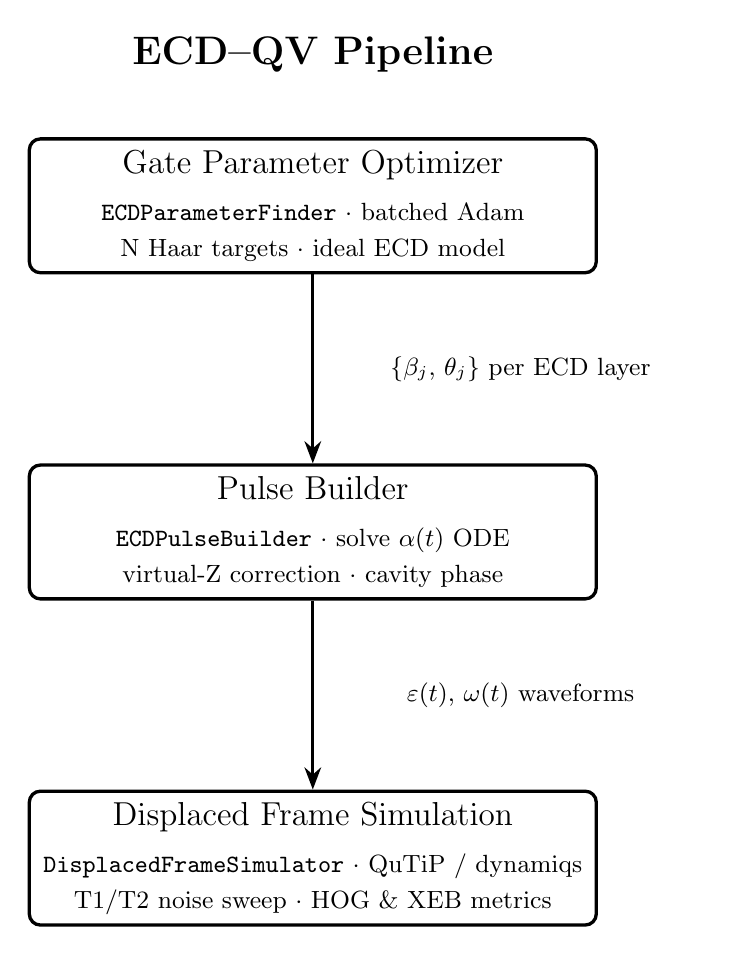
\begin{tikzpicture}[
    box/.style={
        draw, rectangle, rounded corners=4pt,
        minimum width=7.2cm, minimum height=1.7cm,
        align=center, font=\large,
        line width=1.2pt
    },
    arrow/.style={
        ->, -{Stealth[length=8pt]},
        line width=1.2pt
    },
    lbl/.style={font=\small, align=center, text width=4.4cm}
]

\node[font=\Large\bfseries] (title) {ECD--QV Pipeline};

\node[box, below=0.7cm of title] (gate) {
    Gate Parameter Optimizer \\[3pt]
    \small\texttt{ECDParameterFinder} $\cdot$ batched Adam \\[-1pt]
    \small \Nunitaries\ Haar targets $\cdot$ ideal ECD model
};

\node[box, below=2.4cm of gate] (pulse) {
    Pulse Builder \\[3pt]
    \small\texttt{ECDPulseBuilder} $\cdot$ solve $\alpha(t)$ ODE \\[-1pt]
    \small virtual-Z correction $\cdot$ cavity phase
};

\node[box, below=2.4cm of pulse] (sim) {
    Displaced Frame Simulation \\[3pt]
    \small\texttt{DisplacedFrameSimulator} $\cdot$ QuTiP / dynamiqs \\[-1pt]
    \small T1/T2 noise sweep $\cdot$ HOG \& XEB metrics
};

\draw[arrow] (gate.south) -- (pulse.north)
    node[midway, right=0.3cm, lbl] {$\{\beta_j,\,\theta_j\}$ per ECD layer};

\draw[arrow] (pulse.south) -- (sim.north)
    node[midway, right=0.3cm, lbl] {$\varepsilon(t)$, $\omega(t)$ waveforms};

\end{tikzpicture}
\end{document}
